\documentclass[a4j]{jarticle}
\usepackage[dvipdfmx]{graphicx,color}
\usepackage{verbatim}
\usepackage{ascmac}
\usepackage{url}
\usepackage{listings,jlistings}
\usepackage{color}
%\setlength{\marginparwidth}{20mm}%% 傍注欄の横幅の設定

\input{/home/ryousuke/listings_temp.tex}

\title{情報科学プロジェクト実験レポート課題}
\author{S142063 佐藤涼亮}

\begin{document}
\maketitle
\centerline{\LARGE \underline{CGI(Common Gateway Interface)}}
\section{課題の内容}
{\large \underline{CGIプログラムによるWEBインターフェースでのデータベース操作}}
\subsection{要点}
\begin{itemize}
\item C++プログラムをCGIプログラムに修正
\item 第9回目のレポート課題の内容をWEBインターフェースで使えるように変更
\end{itemize}
\section{プログラムの説明}
・郵便番号から住所を検索するプログラム

・住所から郵便番号を検索するプログラム

前回に引き続き以上の2つのプログラムを
Webのインターフェースで使用できるように修正・変更した。
CGIinput.hppは研究室独自のクラスであり、メソッドがGETとPOSTの両方に対応しており、
同一のプログラムとして実装できる。
また、フォームデータを解析して容易に使用できるように実装されている。

\subsection{目的}
Webのインターフェースにおけるデータベースの操作。

\subsection{方法}
CGIプログラムによるデータベースを操作するプログラムの実装。

\subsection{結果}
Webインターフェースで実行した結果をまとめる。

\begin{center}
初期状態
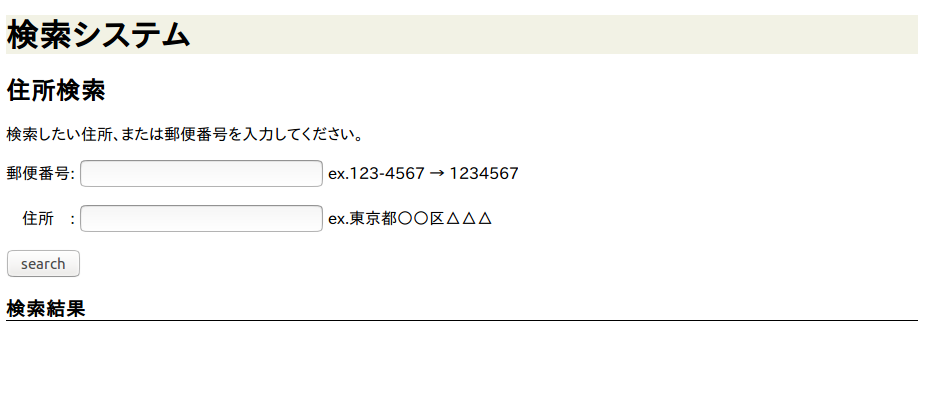
\includegraphics[width=15cm]{result/result1.png}

{\LARGE↓}

郵便番号と住所を入力
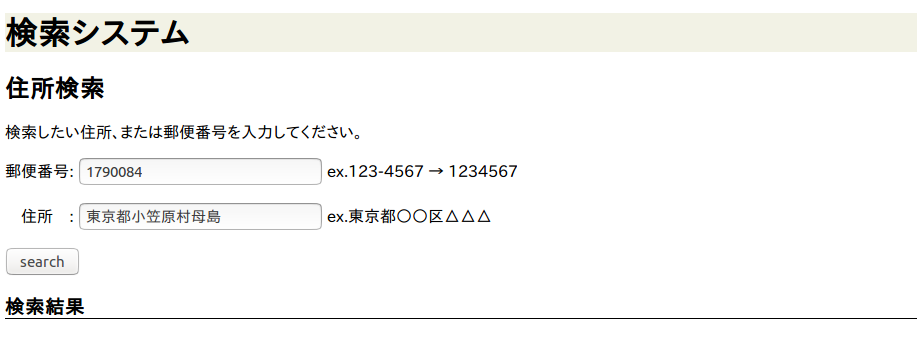
\includegraphics[width=15cm]{result/result2.png}

{\LARGE↓}

searchをクリックすると検索結果が表示される
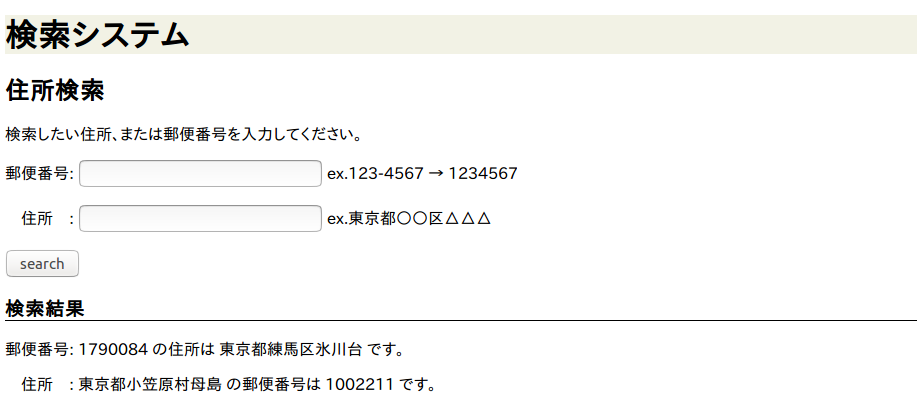
\includegraphics[width=15cm]{result/result3.png}

{\LARGE↓}

郵便番号のみを存在しない値で入力
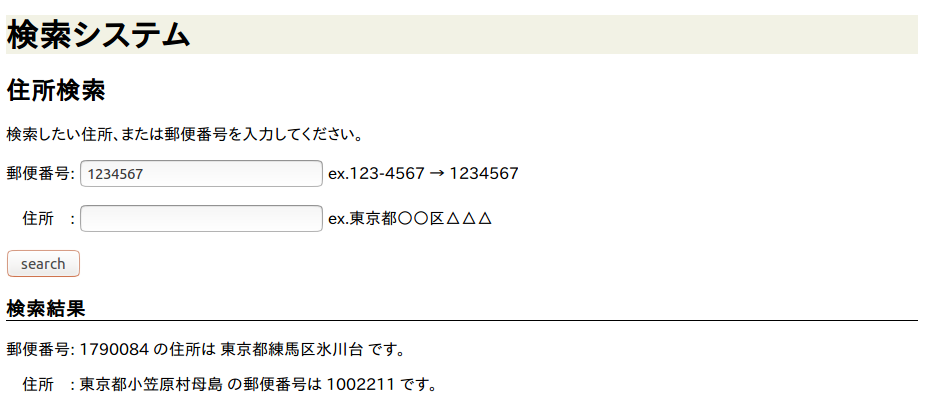
\includegraphics[width=15cm]{result/result4.png}

{\LARGE↓}

入力されなかった住所は何も表示せず\\
入力された郵便番号は存在しないので、一致するものがないと表示

\includegraphics[width=15cm]{result/result5.png}
\end{center}

\subsection{考察}
郵便番号や住所の検索を行うことができ、期待通りの結果が得られた。

\section{感想}
CGIプログラムについて学習した。
今回はC++の言語から作成したが、
CGIプログラムは、いろんなプログラミング言語で作成することができるので、
少し知識のあるperlでも今後扱ってみたい。
そして、情報検索の授業で学習したことと組み合わせて、
Web検索CGIプログラムを作成したい。
また、以前の研究室の課題でもHTML/CSSの学習をしたが、
最近、自主的にHTML/CSSの学習を行っているため、
HTMLと今回の課題は関連性も高く、深く理解することができた。
HTML/CSSの知識を活かし、もっと使用者のことを考え、見やすく扱いやすいように修正してみたい。


\section{プログラム}
\lstinputlisting[caption=report.cpp,label=db.cpp,language=C++]{db.cpp}

\end{document}
